\documentclass[12pt]{article}
\usepackage{amsmath}
\usepackage{amsthm}
\usepackage{amssymb}
\usepackage{enumitem}
\usepackage{graphicx}
\usepackage{hyperref}
\usepackage[margin=1in]{geometry}
\usepackage{times}

\title{Process for Forward Fast Fourier Transform (FFT) Numerical Computation}
\author{}
\date{}

\begin{document}
\maketitle
\subsection*{Overview}
Forward FFT takes time domain data points and converts them to frequency domain coefficients. First it solves for complex numbers ($C_k$), then converts to $a,b$ coefficients for use in partial sums trigonometric interpolation equation. 

\section*{Prerequisites}
\begin{itemize}
    \item $N$ = Number of data points. $N$ must be a power of 2, can zero-pad otherwise. Data points must be evenly spaced on $[-\pi,\pi]$.
    \item $m$ = Degree. Higher solves for higher frequencies in the approximation. $m \leq N/2$
\end{itemize}

\section*{Step 1) Generate Data Points}
For data points $(x_j,y_j)$ on $[-\pi,\pi]$:
\[x_j = -\pi + \frac{2\pi j}{N}, \quad j=0,1,\ldots,N-1\]
\[y_j = f(x_j), \quad j=0,1,\ldots,N-1\]

\section*{Step 2) Pre-compute setup values:}
\subsection*{a) Pre-computed "Roots of Unity":}
\[W_k = e^{-2\pi ik/N} = \cos(2\pi k/N) - i\sin(2\pi k/N), \quad k=0,1,\ldots,(N/2)-1\]
\\
Note: Only need to compute each $W_k$ once.\\
Note: $W$ values "loop" around a unit circle for higher values.\\
\begin{align*}
\text{ex: } N=8&, \text{with } \log_2(8)= 3: \\
W_0 &= e^{-2\pi i(0)/8} = 1.0000+0.0000i &(0^\circ)\\
W_1 &= e^{-2\pi i(1)/8} = 0.7071-0.7071i &(45^\circ)\\
W_2 &= e^{-2\pi i(2)/8} = 0.0000-1.0000i &(90^\circ)\\
W_3 &= e^{-2\pi i(3)/8} = -0.7071-0.7071i &(135^\circ)\\
\cline{1-3}\\
W_4 &= -W_0 = -1.0000+0.0000i &(180^\circ)\\
W_5 &= -W_1 = -0.7071+0.7071i &(225^\circ)\\
...
\end{align*}

Loop rules:
\begin{itemize}
    \item $W_{k+4} = -W_k$ (opposite side of circle)
    \item $W_{k+8} = W_k$ (full rotation)
\end{itemize}

\subsection*{b) Initial complex values array:}
\begin{enumerate}[label=\roman*)]
    \item Set initial complex values to y values:
    \[C_j = y_j, \quad j=0,1,\ldots,N-1\]
    \item Bit-reverse the complex values index positions so butterfly pairing is correct.\\
    For array size $N$, each index $i$ (for 0 to $N-1$) is found by:
    \begin{enumerate}
        \item Convert to binary in $\log_2(N)$ bits
        \item Reverse the bits
        \item Convert back to decimal
        \item Re-order complex pairs with new index
    \end{enumerate}
\end{enumerate}

Ex: $N=8$, with $\log_2(8)=3$ bits:
\begin{center}
\begin{tabular}{|c|c|c|c|}
\hline
i & binary & reversed & new i\\
\hline
0 & 000 & 000 & 0\\
1 & 001 & 100 & 4\\
2 & 010 & 010 & 2\\
3 & 011 & 110 & 6\\
4 & 100 & 001 & 1\\
5 & 101 & 101 & 5\\
6 & 110 & 011 & 3\\
7 & 111 & 111 & 7\\
\hline
\end{tabular}
\end{center}

\[C_0 \to C_0, C_1 \to C_4, C_2 \to C_2, C_3 \to C_6, \text{ etc.}\]
Note: Only need to compute bit-reversal index table once.

\section*{Step 3) Butterfly Pairs}
Combine complex values in pairs over stages, updating values one step at a time, until the final complex values are fully computed. Pairs of $C_k$ are found by increasing the distance when grouping the arrays:
\begin{itemize}
    \item Stage Number: $s = 1,2,\ldots,\log_2(N)$
    \item Distance between pairs in stage: $d = 2^{s-1}$
\end{itemize}

$ $\\
For example, with $N=8$ and $\log_2(8)=3$ stages:
\begin{align*}
\text{Stage 1 (distance = 1):} & \quad [0],[1],[2],[3],[4],[5],[6],[7] \to \{(0,1),(2,3),(4,5),(6,7)\}\\
\text{Stage 2 (distance = 2):} & \quad [0,1],[2,3],[4,5],[6,7] \to \{(0,2),(1,3),(4,6),(5,7)\}\\
\text{Stage 3 (distance = 4):} & \quad [0,1,2,3],[4,5,6,7] \to \{(0,4),(1,5),(2,6),(3,7)\}
\end{align*}
$ $\\
For each pair, perform the following ($N$ = total \# of points, $d$ = distance between pairs):
\begin{align*}
\eta &= C_{k+d} \times W_{(k\times N/2d)}\\
C_k &= C_k + \eta\\
C_{k+d} &= C_k - \eta
\end{align*}

\section*{Step 4) Coefficient Extraction}
Convert complex values to $a_k$ and $b_k$ values:
\[a_0 = \frac{1}{N}Re(C_0)\]

\[-a_k = \frac{2}{N}Re(C_k) \quad \quad b_k = \frac{2}{N}Im(C_k) \quad \text{, for odd } k=1,3,\ldots,(N/2)-1\]

\[a_k = \frac{2}{N}Re(C_k) \quad \quad -b_k = \frac{2}{N}Im(C_k) \quad \text{, for even } k=2,4,\ldots,(N/2)-1\]

\[a_{N/2} = \frac{1}{N}Re(C_{N/2}), \quad \text{for } k = N/2\]

\section*{Step 5) Construct Fourier series approximation}
Interpolating Polynomial Equation for FFT:
\[S_m(x) = \frac{a_0 + a_m\cos(mx)}{2} + \sum_{k=1}^{m-1}(a_k\cos(kx) + b_k\sin(kx))\]

\section*{Numerical Computation Implementation}
To validate the FFT process above was correct we implemented it from scratch in p5.js, creating an interactive web interface on top that allows users to analyze arbitrary functions. User selected functions are sampled at $N$ points between $-\pi$ and $\pi$, our FFT computes the complex coefficients and derives the $a_k$ and $b_k$ coefficients. Those coefficients are used to construct the Fourier series partial sum approximation, which is then graphed below the original function for comparison. The magnitude of each coefficient calculated and displayed on the bottom. The user can either select from predefined functions or input custom functions, and adjust the $N$ sampling resolution. \\
\\
\textbf{Click Play icon in top left to run the app:} \\
\url{https://editor.p5js.org/travisformayor/sketches/by5UTP__f}

\begin{figure}[htbp]
\centering
\begin{tabular}{cc}
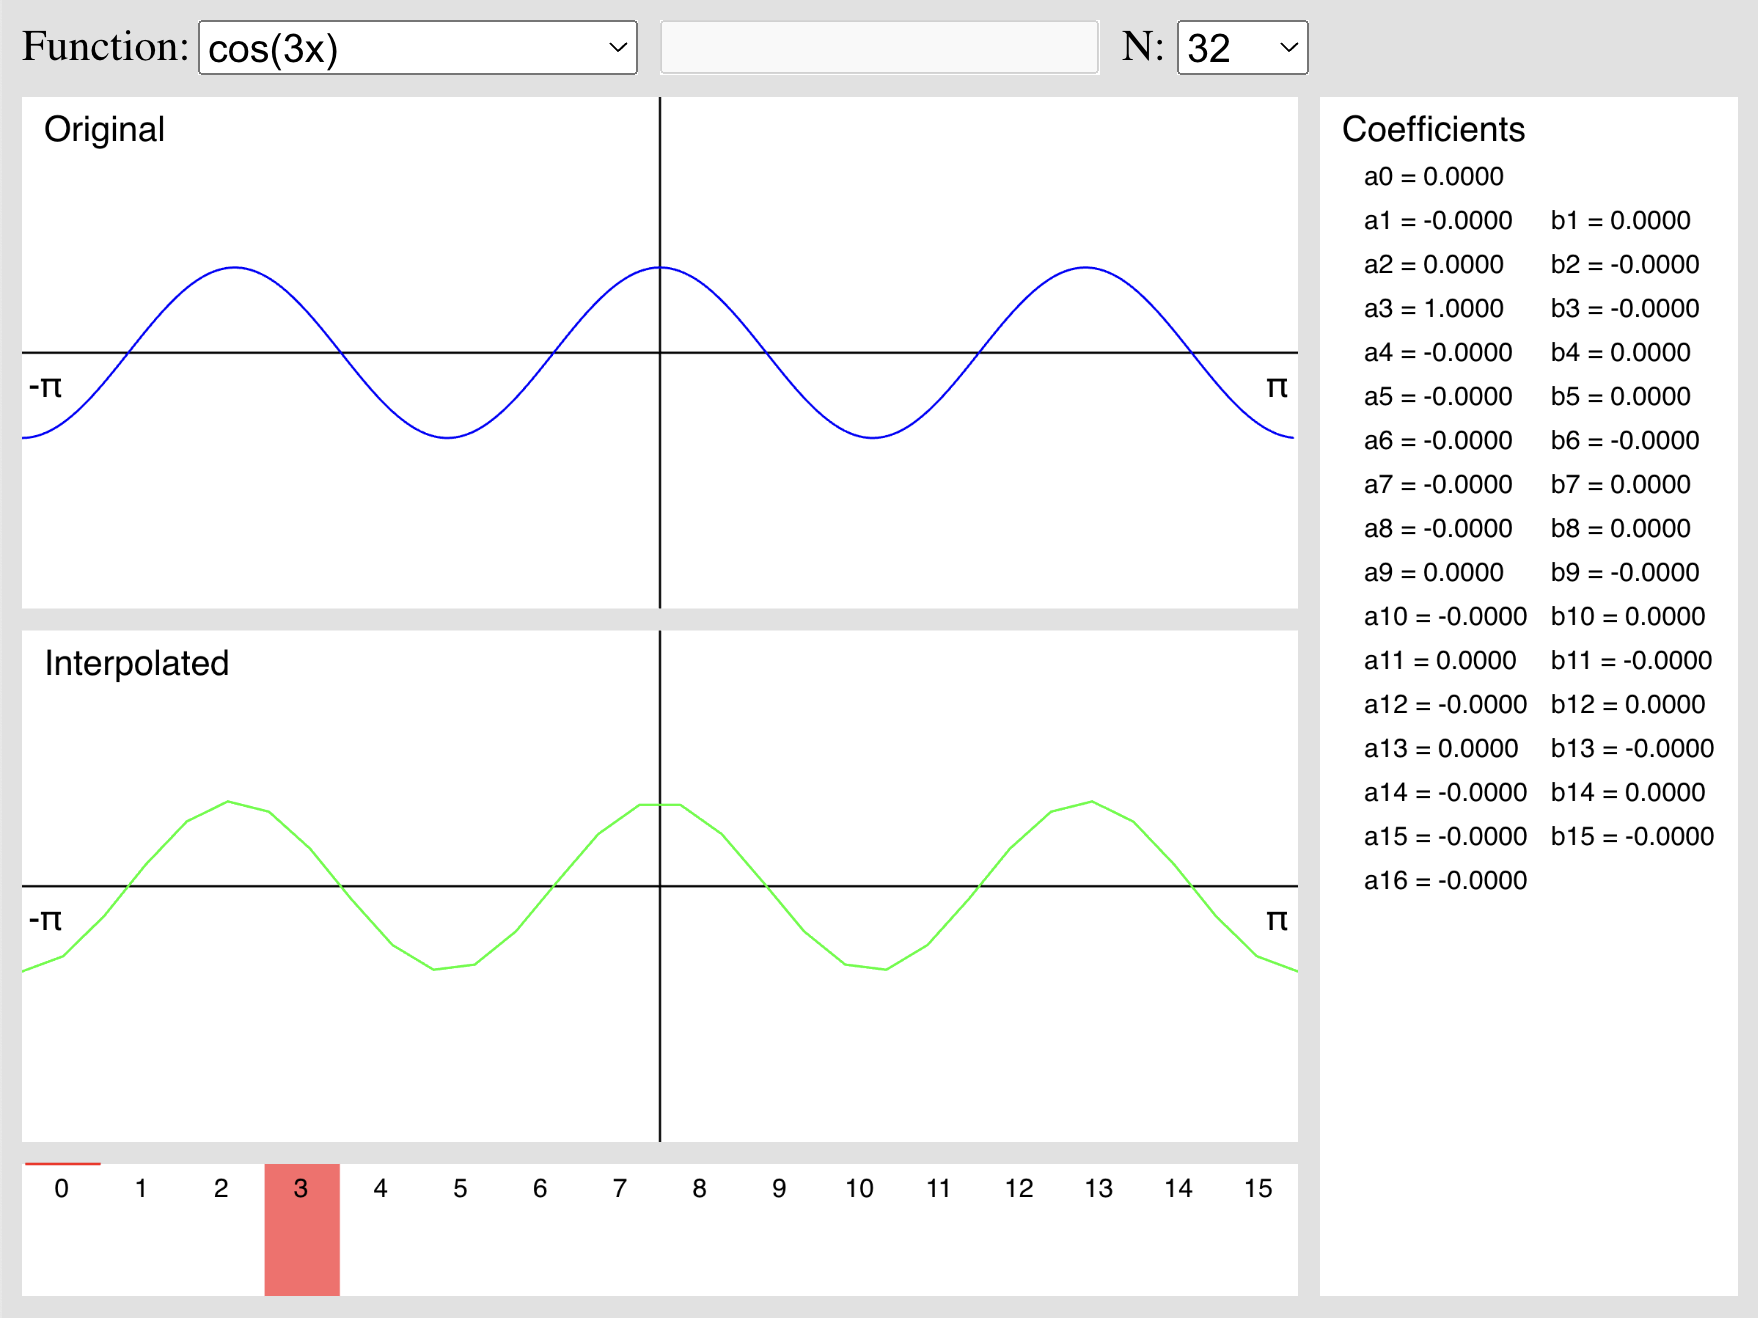
\includegraphics[width=0.45\textwidth]{img-cos3x.png} &
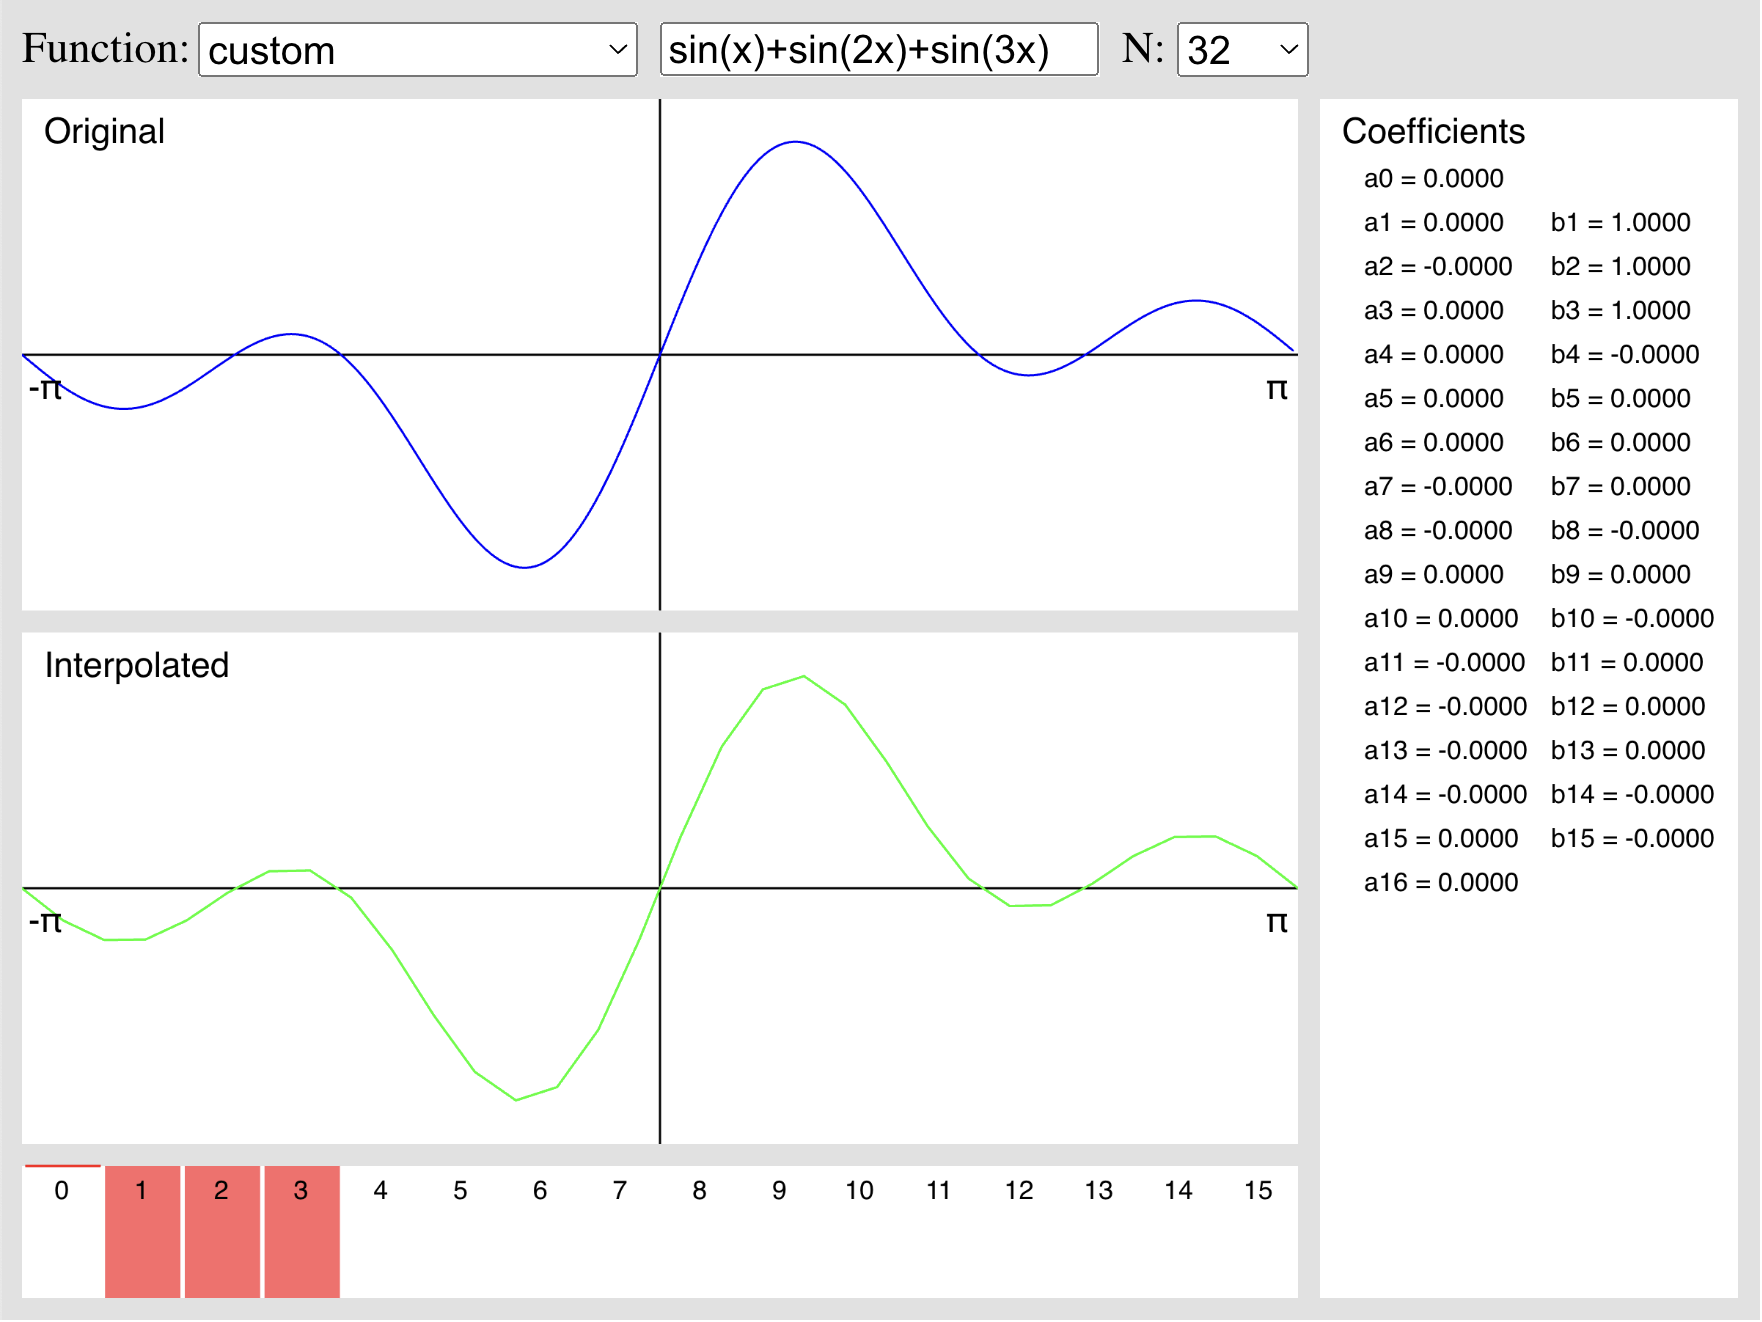
\includegraphics[width=0.45\textwidth]{img-custom.png} \\ [-5pt]

{\footnotesize $f(x) = cos(3x)$} & 
{\footnotesize $f(x) = sin(x)+sin(2x)+sin(3x)$} \\ [-2.5pt]

{\footnotesize Notice 3rd spectrum.} &
{\footnotesize Notice 1, 2, and 3 spectrums.} \\[10pt]

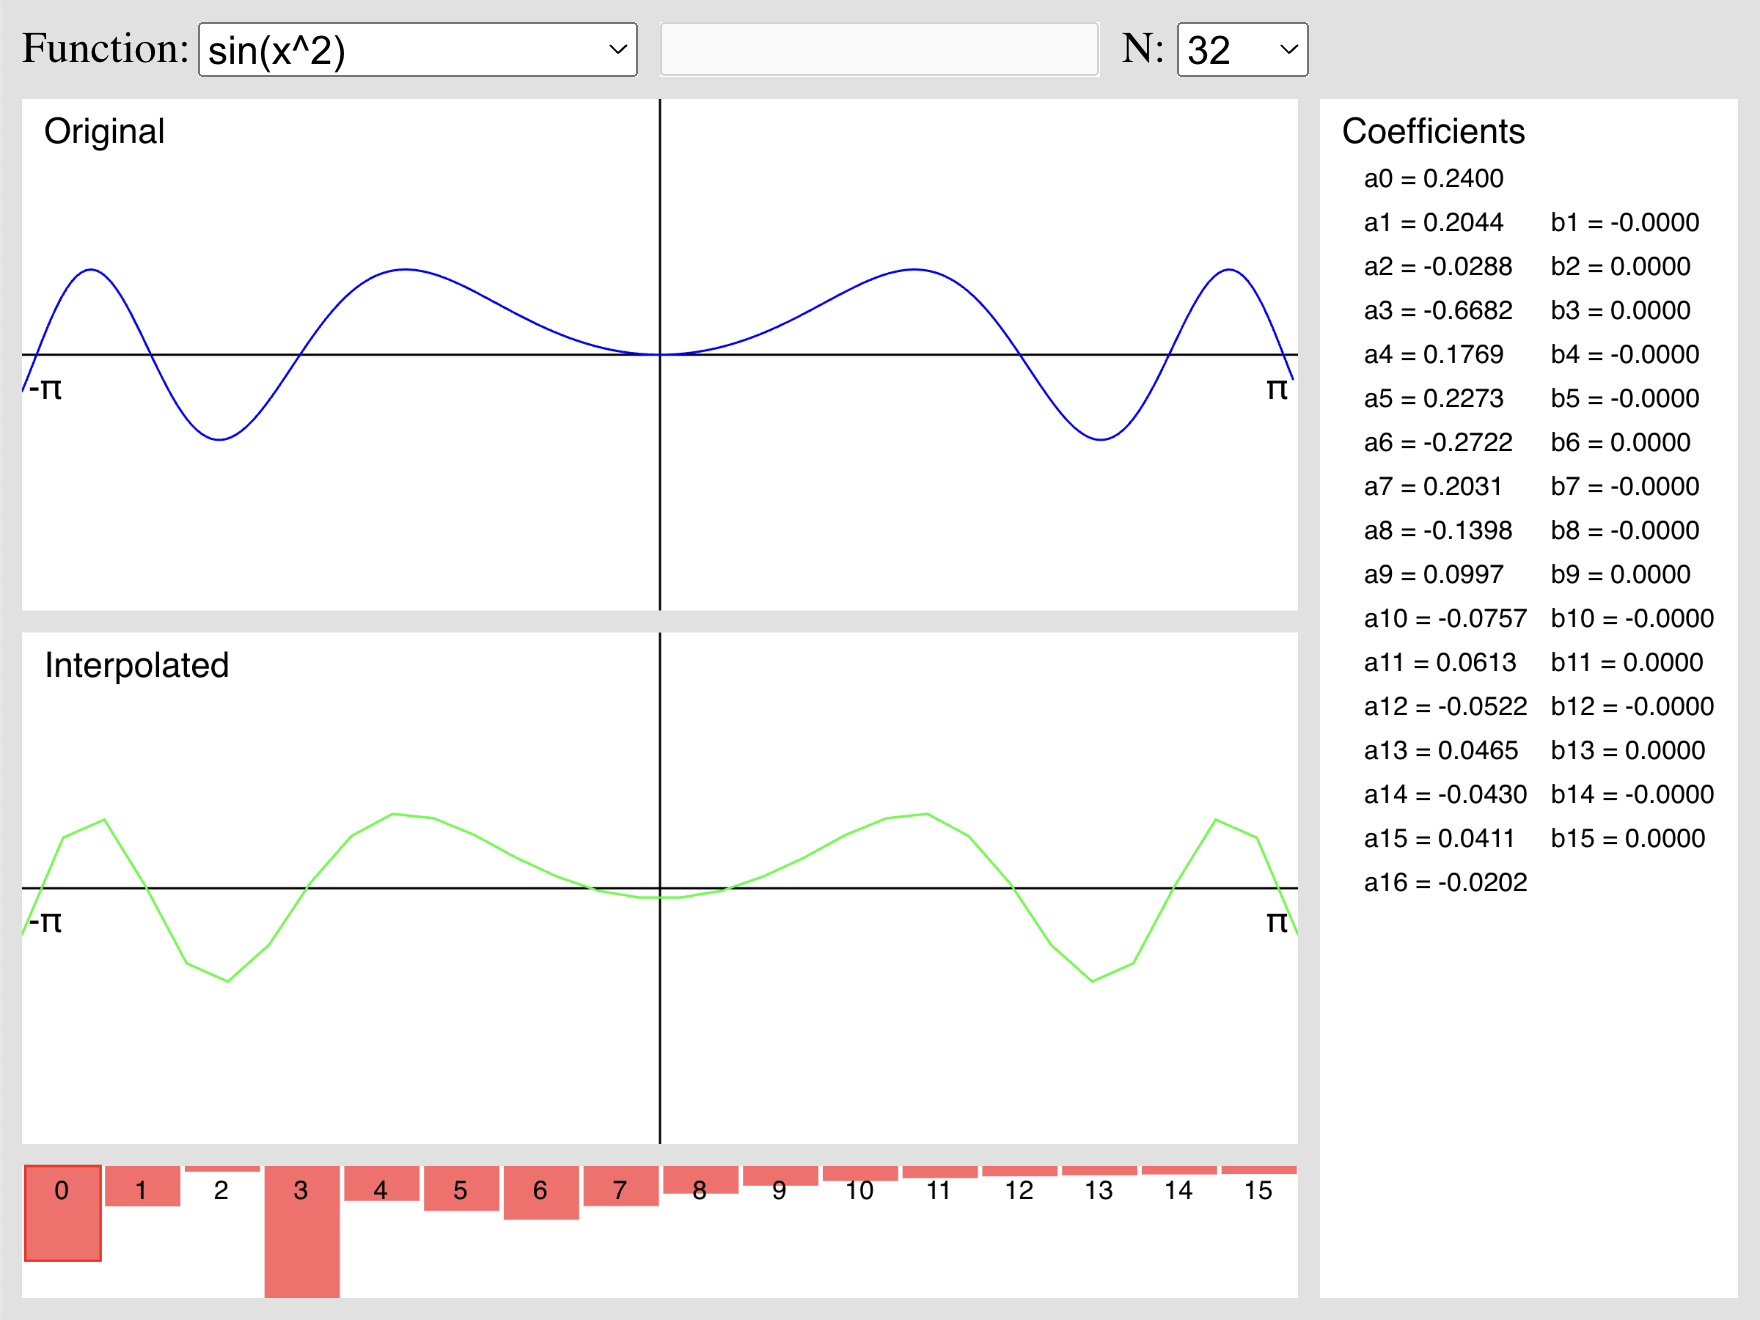
\includegraphics[width=0.45\textwidth]{img-sinx2.png} & 
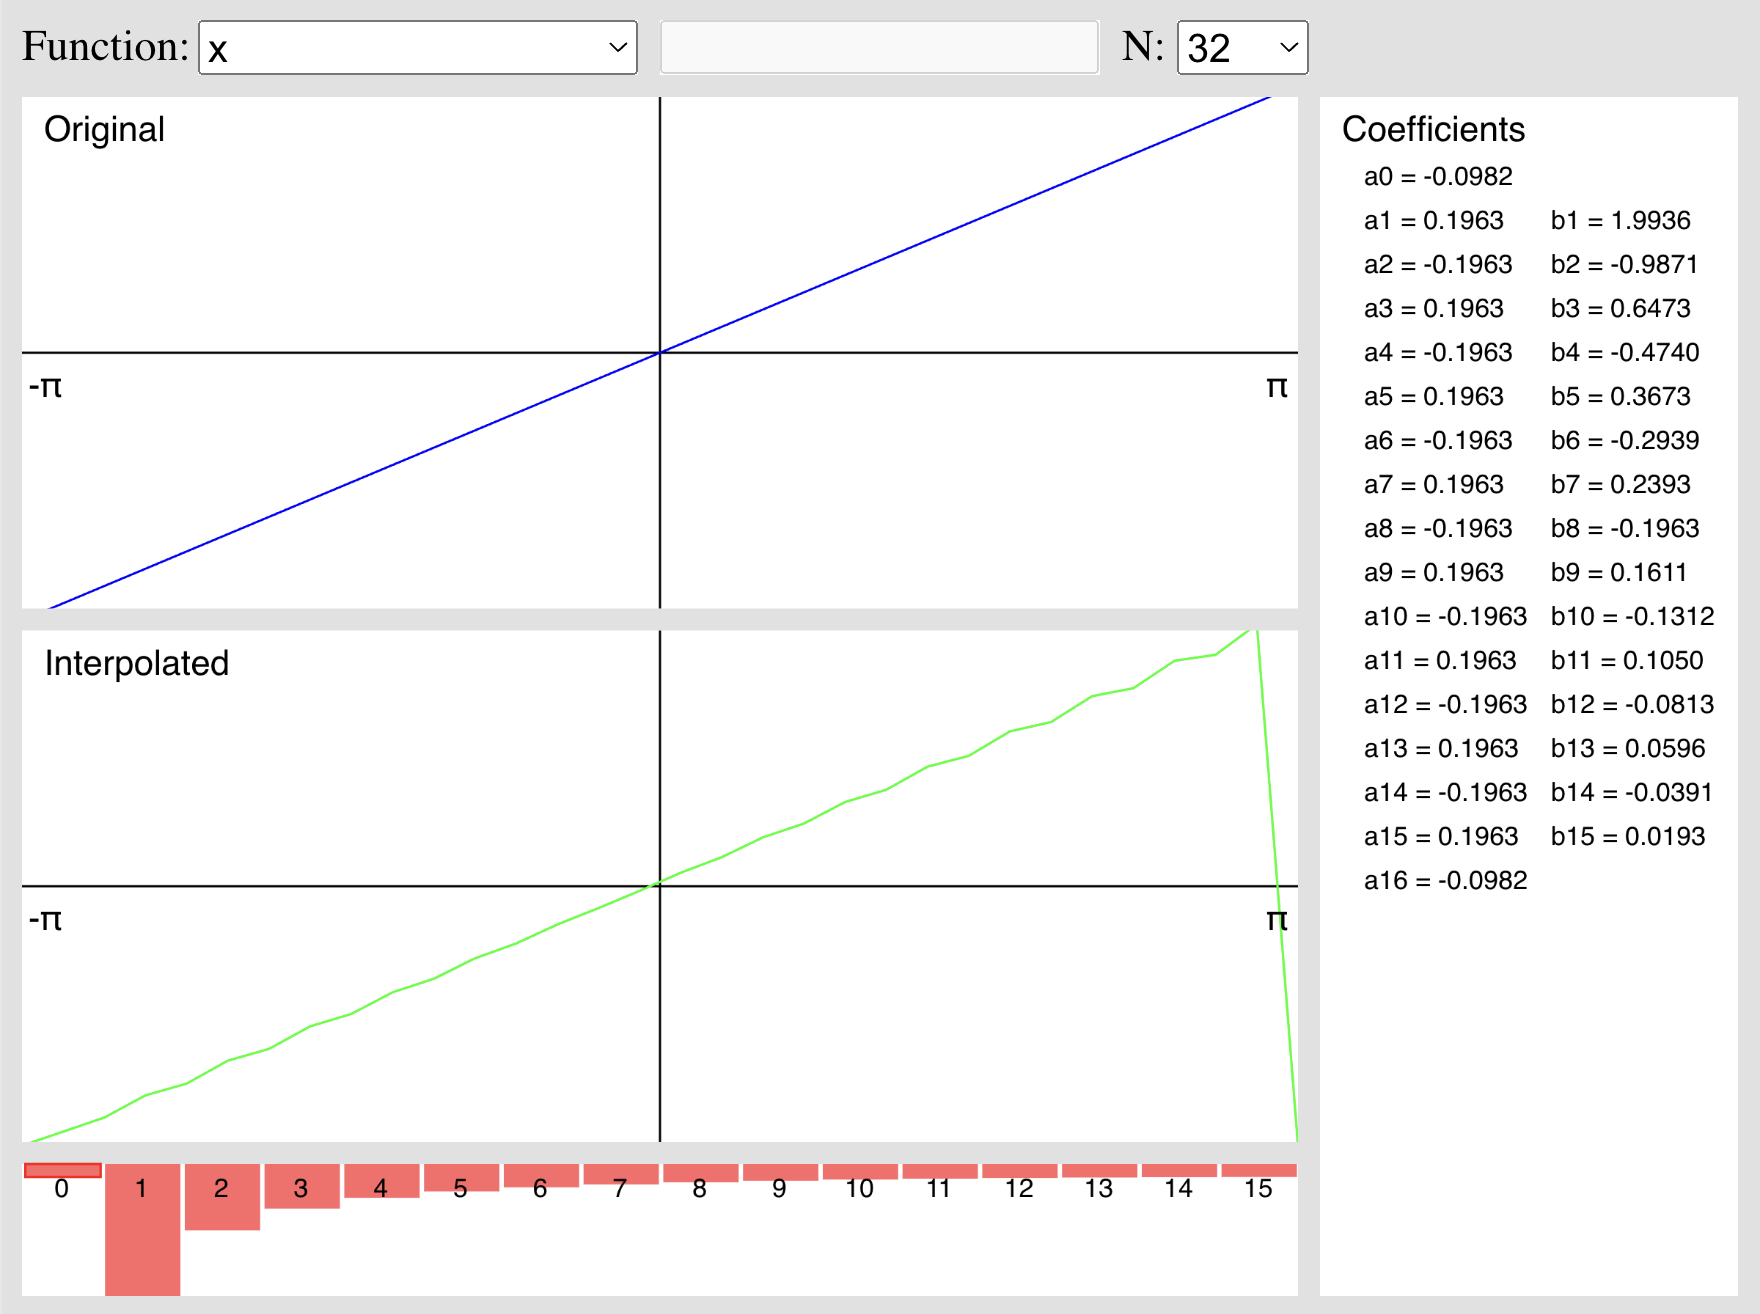
\includegraphics[width=0.45\textwidth]{img-x.png} \\ [-5pt]

{\footnotesize $f(x) = sin(x^2)$} & 
{\footnotesize $f(x) = x$} \\ [-2.5pt]

{\footnotesize } &
{\footnotesize Notice the break on the end. See below for more } \\[-2.5pt]
{\footnotesize } &
{\footnotesize information on the Gibbs Phenomenon.} \\[10pt]

\end{tabular}
\end{figure}

Gibbs Phenomenon occurs near points in a Fourier transformation involving a complete revolution of the unit circle. Since FFT trigonometric interpolation is constructed using a combination of sine and cosine functions to create a best fit, it utilizes the periodicity of the unit circle ($2\pi$ to make a complete revolution) and, therefore, has large jumps at points of discontinuity. Take, for example, the function $f(x) = x$ (pictured above). Since $x$ is not periodic and is instead monotonically increasing, once the interpolation of the function nears points that are a multiple of $\pm \pi$, the natural periodicity of the sine and cosine functions being used to make the best fit of the function have a huge jump as they attempt to "reset" to their negative side of the unit circle. This does not happen to functions in the program that are periodic, such as $\sin(x)$, $\cos(x)$, $x^2$, or $|x|$, but other examples where it does occur would be any constant times $x$ ($2x$, $3x$, ...), $e^x$, or $x$ to an odd degree ($x^3$, $x^5$, ...).

\end{document}